\addcontentsline{toc}{chapter}{Introduction}
\chapter*{Introduction}
	Durant cette série de travaux pratiques, il nous a été demandé de mettre en place une implémentation du métamodèle d'architecture à base de composants développé lors des précédentes séances. Ce métamodèle (niveau \emph{M$2$} ; nommé \emph{HADL} dans le cadre de ce projet), devait pouvoir être instancié en n'importe quel type de modèle d'architecture (niveau \emph{M$1$}). Le modèle architecturale obtenu doit pouvoir être lui-même instancié (niveau \emph{M$0$})
    \newline
    
    La création et la réflexion autour de l'organisation de ce métamodèle a donné lieu à un précédent rapport décrivant précisément la modélisation retenue ainsi que nos choix du point de vue de l'abstraction. Il liste les concepts essentiels ainsi que les interactions possibles.
    \newline
    
    Dans ce présent rapport, nous nous pencherons sur l'outil que nous avons développé. Cet outil permet, entre autres, de représenter un modèle à base de composant, d'instancier ce modèle et de simuler le fonctionnement des services des différents composants.
    \newline
    
    Ce papier s'organisera autours de cinq axes majeurs :
    ~\\
    \begin{itemize}
    	\item un rappel des entités principales de notre métamodèle
        \item l'implémentation de ces concepts
        \item le gestionnaire de services
        \item la vérification de l'architecture
        \item l'exemple client-serveur
    \end{itemize}
	~\\
    Nous concluerons ce rapport en évoquant les possibilités de développement futures autour de notre outil, les limites actuelles et les difficultés rencontrées.
    
\chapter{Métamodèle}

    Le métamodèle de notre application repose sur deux concepts fondamentaux : les entités et les relations. Cette section rappellera brièvement ces points clés, les avantages et les inconvénients d'une telle modélisation. Pour en avoir une description plus approfondie, nous vous recommendons notre précédent document.
    
    \section{Rappel des éléments de base}
    	
        \emph{HADL} repose sur trois concepts principaux qui forment le c\oe{}ur de la représentation architecturale : 
        \begin{itemize}
        	\item \textbf{Les composants :} briques logicielles de base de l'application
            \item \textbf{Les connecteurs :} permettent l'interconnexion entre les composants
            \item \textbf{Les configurations :} permettent de définir des conteneurs de composants/connecteurs
        \end{itemize}
        
        Dans notre modélisation, les configurations permettent de définir un modèle sur plusieurs niveaux de granularités : une configuration peut elle-même contenir (indirectement) une configuration \ldots
        \newline
        
        Toutes ces entités fournissent un ensemble d'interfaces, définissants leurs besoins et leurs productions. Ces interfaces sont la base de l'interconnexion entre entités.
        \begin{itemize}
        	\item Les composants fournissent deux types d'interfaces
            \begin{itemize}
            	\item \textbf{Des ports} fournis et requis
                \item \textbf{Des services} fournis et requis
            \end{itemize}
            \item Les connecteurs fournissent un seul type d'interface : \textbf{les roles}
        \end{itemize}
        
        Les configurations fournissent tour à tour les interfaces des composants ou des connecteurs, en fonction du type d'entité qu'elles représentent.
        \newline
        
        Les entités de bases seules ne permettent pas de représenter une architecture digne de ce nom. Pour cela il est nécessaire de définir les liaisons entre les composants, connecteurs et configurations. Dans \emph{HADL}, nous avons défini deux types de liens :
        \begin{itemize}
        	\item \textbf{Les attachments :} liens "horizontaux" entre les composants et les connecteurs. Ces liens permettent de définir les interactions sur un niveau de granularité donné.
            \item \textbf{Les bindings :} liens "verticaux" entre les configuration et les composants/connecteurs qu'elles contiennent. Ces liens permettent de déléguer des comportement dans la représentation interne d'une configuration ou d'en extraire un résultat.
        \end{itemize}
        
	\section{Avantages}
    
    	Le principal avantage de notre modélisation est son exhaustivité : elle permet de représenter tous les concepts vus durant les cours de \emph{CSA}. Les liens sont séparés en deux sous-concepts, qui permettent de faire abstraction de la granularité (pour les \emph{attachment}) ou de la largeur (pour les \emph{bindings}).
        \newline
        
        Comme les concepts de notre langage sont bien séparés (par exemple les ports/roles des configurations ne sont pas les mêmes que ceux des composants/connecteurs), il n'y a pas d'ambiguïté lorsque l'on souhaite décrire une architecture complexe. De plus, cette organisation permet de facilement organiser le \emph{runtime} en spécifiant divers comportements en fonction de l'élément considéré. Cet aspect de notre application sera décrite dans le chapitre \ref{runtime-chapter}. 
        
	\section{Inconvénients}
    	Du fait du grand nombre de concepts contenus dans notre métamodèle, il peut être difficile à appréhender. Par exemple, la différence entre les ports des composants et des configurations n'est pas intuitive.
        \newline
        
        Comme expliqué dans le précédent document, il nous a été difficile de mettre en place notre métamodèle, en particulier extraire certains concepts, ou encore limiter les interactions entre concepts (par exemple les bindings ne peuvent se faire que sur deux niveaux adjacents).
        
	\section{Instanciation}
    	Dans notre précédent document, nous avons détaillé l'instanciation d'un modèle \emph{client-serveur} à partir de notre métamodèle. Ce modèle permet de mettre en \oe{}uvre une grande partie des fonctionnalités demandées (composants, connecteurs, configuration, points de vues sur plusieurs niveaux avec \emph{bindings}, liaisons avec \emph{attachments}).
        \newline
        
        Nous nous servirons de cette exemple d'utilisation de notre métamodèle dans le dernier chapitre (\ref{cs-chapter}) de ce rapport pour montrer l'utilisation de l'outil que nous avons développé.
        
\chapter{Application}
\label{application-chapter}

	Dans le chapitre précédent, nous avons fait un bref rappel des concepts essentiels de notre métamodèle, les avantages ainsi que les inconvénients de notre modélisation. Dans ce chapitre, nous nous intéresserons à l'implémentation de notre outil. Dans un premier temps nous détaillerons la partie statique de notre métamodèle. Nous étudierons ensuite la gestion des liaisons. Enfin, nous ferons une brève analyse des différence entre notre modèle au niveau conceptuel et au niveau de l'implémentation.
    
    \section{Généralités}
      Nous avons choisi de développer notre outil en utilisant le langage \emph{java}. Etant familiers avec ce langage et avec la structuration qu'il propose (classes, packages, abstractions \ldots) nous l'avons jugé adapté à notre outil.
      \newline
      
      Notre application est décomposée en deux modules (packages) principaux :
      \begin{itemize}
      \item \textbf{M2} : contient l'ensemble des classes représentant notre métamodèle (y compris les classes de \emph{runtime} et de vérifications)
      \item \textbf{M1} : un exemple d'utilisation de notre métamodèle, reprenant l'exemple du modèle client serveur du précédent rapport
      \end{itemize}
      ~\\
      Dans ce chapitre, nous nous intéresserons seulement au package  \textbf{M2}, en excluant les sous-modules concernant l'exécution et la vérification (ces modules seront respectivement abordés dans les chapitre \ref{runtime-chapter} et \ref{checker-chapter}).
      
	\section{Entités}
    	Les entités de base de notre métamodèle sont représentées par des classes abstraites. Les relations de compositions présentes dans notre métamodèle ont été scrupuleusement suivies.
        
        \subsection{Composants}
        	La classe \emph{Component} représente un composant. Un composant possède plusieurs propriétés :
            \begin{itemize}
            	\item un nom, représenté par une chaîne de caractères
                \item une configuration parente (qui contient le composant)
                \item une sous-configuration (cas des composants composites)
                \item deux ensembles de ports (fournis et requis)
                \item deux ensembles de services (fournis et requis)
            \end{itemize}
            ~\\
            
            Nous avons fait le choix de représenter les ports fournis et requis par une unique classe \emph{ComponentPort}. L'accès aux différents types de ports se fait par les méthodes dédiées \lstinline{getProvPort()} et \lstinline{getReqPort()}. Cette représentation permet d'alléger et de rendre plus compréhensible l'implémentation de notre métamodèle.
            \newline
            
            Dans notre modélisation, un composant ne peut pas exister seul : il est obligatoirement contenu dans une configuration. Cette restriction a été mise en place car l'ensemble de la logique d'exécution et de création de liens se situe dans les configuration.
            \newline
            
            La sous-configuration (initialement nulle) permet de définir un composant composite. Cette configuration peut représenter tout ou partie de la structure interne du composant. Il est à noter qu'un composant ne peut contenir plus d'une configuration interne.
            
		\subsection{Connecteurs}
        	La classe \emph{Connector} représente un connecteur. Elle possède un certain nombre de propriétés, relativement proches de celles d'un composant :
            \begin{itemize}
            	\item un nom
                \item une configuration parent (contenant le connecteur)
                \item une sous-configuration (cas des connecteurs composites)
                \item deux ensembles de rôles (\emph{from} et \emph{to})
                \item une glue (logique interne du connecteur)
            \end{itemize}
            ~\\
            
            Comme pour le composant, nous avons fait le choix de représenter les rôles \emph{from} et \emph{to} par une unique classe \emph{ConnectorRole}. L'accès aux différents types de rôle se fait, comme pour les composants, par les méthodes dédiées \lstinline{getFromRole()} et \lstinline{getToRole()}.
            \newline
            
            A l'instar des composants, les connecteurs ne peuvent exister seuls et doivent obligatoirement être déclaré dans une configuration.
            \newline
            
            La glue du connecteur permet de représenter la logique même du connecteur : transformer les données en entrée pour qu'elles correspondent aux format attendu en sortie. Cette glue n'est présente que dans le cas de connecteurs atomiques. La logique de connexion des connecteurs composites est contenue dans la sous-configuration.
            
		\subsection{Configuration}
        	La classe \emph{Configuration} représente un conteneur de composants et connecteurs. Cette classe constitue la classe centrale de notre implémentation, puisqu'elle contient l'ensemble des informations de liens entre les composants et les connecteurs qu'elle contient.
            Elle partage également un ensemble de propriétés avec les composants et les connecteurs : 
            \begin{itemize}
            	\item un nom
                \item un parent (cas des composants/connecteurs composites)
                \item un ensemble de composants (les composants qu'elle contient)
                \item un ensemble de connecteurs (les connecteurs qu'elle contient)
                \item un ensemble de liens "horizontaux" (\emph{attachments})
                \item un ensemble de liens "verticaux" (\emph{bindings})
            \end{itemize}
            ~\\
            
            Le parent d'une configuration correspond au composant ou connecteur qu'elle décrit. Ce parent peut être laissé nul (cas de la configuration représentant l'application dans son ensemble).
            \newline
            
            Les ensemble de composants et de connecteurs correspondent aux composants et connecteurs directement inclus dans la configuration. On peut noter qu'une configuration ne peut pas explicitement contenir une autre configuration. Ces sous-configurations peuvent être obtenus via les composants et connecteurs internes (en leur affectant une sous-configuration). L'objectif est de forcer l'utilisateur à définir le type de configuration qu'il souhaite manipuler (composant ou connecteur).
            \newline
            
            Les liens contenus dans une configuration concernent directement les niveaux architecturaux adjacents à la configuration. Plus clairement, une configuration prend en charge les liaisons entre ses composants/connecteurs ainsi que les \emph{bindings} vers ces derniers et vers son éventuel parent.
            
            Nous détaillerons dans la prochaine section la gestion des liens que nous avons mis en place.
            \newline
            
            En plus de ces propriétés, les configurations peuvent contenir un ensemble de ports/services ou de rôles, en fonction de l'entité qu'elles décrivent. Ces deux types d'interfaces ne sont pas compatibles (une configuration ne peut pas représenter à la fois un composant et un connecteur).
            
            Nous avons choisi de garder la différenciation entre les ports/service et rôles des configurations des autres entités. Cette différenciation est essentielle pour la restrictions du champ d'application des liens que nous verrons dans la prochaine section.
            
	\section{Liens}
    
    	Les liens de notre métamodèle sont représentés par des classes finales dans notre application. En effet, les liens ne sont pas dépendants de l'implémentation et n'ont donc aucune raison d'être sous-classés.
        
        Les contraintes sur les champs d'applications des liens de notre métamodèle ont également été scrupuleusement suivies afin d'éviter que notre outil puisse représenter des modèles incohérents.
        
        \subsection{Attachment}
        	La classe \emph{Attachment} représente les liens "horizontaux". Ces liens permettent de relier entre-elles des entités d'un même niveau architectural (dans la même configuration).
            \newline
            
            Comme nous l'avons décrit dans notre précédent rapport, ces liaisons ne peuvent être créées que sous certaines conditions :
            \begin{itemize}
            	\item les entités à relier ont le même niveau architectural
            	\item les entités à relier sont un port (d'un composant) et un rôle (d'un connecteur)
                \begin{itemize}
                  \item si le port du composant est un port fourni alors le rôle du connecteur doit être un rôle \emph{from}
                  \item si le port du composant est un port requis alors le rôle du connecteur doit être un rôle \emph{to}
                \end{itemize}
            \end{itemize}
            ~\\
            
            On peut noter que ces contraintes interdisent tout type de liaison horizontales mettant en jeu une configuration. Ce comportement est souhaité, comme nous l'avons expliqué précédement, toute configuration peut être déclarée comme décrivant un composant et un connecteur (sur lesquels les \emph{attachments} sont possibles). De plus, comme les configurations contiennent les \emph{attachments} des entités qu'elle contient, et qu'une configuration ne peut directement en contenir une autre, permettre ce type de liaison n'avait pas de sens.
            \newline
            
            Les contraintes sur les types de ports/rôle permettent de restreindre encore la création de ces liens, en ne gardant que les situations valides. Il n'est donc pas possible dans notre application de relier directement deux composants, même si leurs interfaces correspondent. Pour mettre en place une telle architecture il suffit d'utiliser un connecteur effectuant une identité entre ses rôles d'entrée et de sortie.
            
		\subsection{Bindings}
        	La classe \emph{Binding} représente les liens "verticaux". Ces liens permettent de relier une configuration avec les niveaux architecturaux autour d'elle (supérieur et inférieur). Comme pour les \emph{attachments}, la classe \emph{Binding} est finale car non dépendante du modèle qu'elle représente.
            \newline
            
            Tout comme les \emph{attachments}, ces liaisons ne peuvent être créées que sous certaines conditions :
            \begin{itemize}
            	\item les entités à relier sont adjacentes d'un point de vue architectural
                \item les entités à relier sont un port (d'un composant) et un port (d'une configuration) ou un rôle (d'un connecteur) et un rôle (d'une configuration).
                \begin{itemize}
                  \item si le port du composant est un port fourni alors le port de la configuration doit être un port fourni
                  \item si le port du composant est un port requis alors le port de la configuration doit être un port requis
                  \item si le rôle du connecteur est un rôle \emph{from} alors le rôle de la configuration doit être un rôle \emph{from}
                  \item si le rôle du connecteur est un rôle \emph{to} alors le rôle de la configuration doit être un rôle \emph{to}
                \end{itemize}
            \end{itemize}
            ~\\
            
            Ces contraintes permettent de représenter tous les liens verticaux entre une configuration et son contenu, ainsi qu'entre une configuration et l'entité qui la contient. Les contraintes sur les types de rôles/ports assurent qu'une configuration ne peut ni déléguer, ni faire remonter des informations provenant d'un autre type d'interface que celles de son parent.
            
	\section{Analyse}
    	Comme nous l'avons expliqué tout au long de ce chapitre, nous avons essayé de coller au plus près du métamodèle que nous avons défini précédement.
        \newline
        
        Néanmoins, nous avons utilisé certaines facilités de la programmation objet afin de réduire le nombre de classes utilisées. Nous n'avons par exemple pas différencié les interfaces fournies et requises ou les rôles \emph{from} et \emph{to} au niveau classes. Comme expliqué précédement, cette différenciation est faites par les méthodes d'accès.
        \newline
        
        Nous avons gardé les contraintes imposées par le métamodèle, il a cependant fallu les adapter au niveau du codage, en particulier car la différence entre les ports requis et fournis n'était plus de l'ordre de la classe, mais une propriété liée au composant contenant le port.
        
\chapter{Runtime}
\label{runtime-chapter}

	Dans le chapitre précédent, nous avons vu comment nous avons transposé notre métamodèle en un ensemble de classes et de relations java. Ce chapitre détaillera un point essentiel de notre outil : le \emph{runtime}. Nous verrons dans un premier temps le champ d'application ainsi que les classes impactées par ce runtime. Nous nous pencherons ensuite sur son fonctionnement et ses limites.
    
    \section{Généralités}
    	Le \emph{runtime} de notre outil correspond à la propagation des valeurs des ports et des rôles. Il permet de simuler le transfert d'informations lorsqu'un service est appelé.
        \newline
        
        Au niveau développement, nous avons choisi d'utiliser la surcouche du langage java \emph{AspectJ}. Ce langage nous permet d'utiliser la programmation par aspects, particulièrement bien adapté à cette situation (le \emph{runtime} agit sur presque toutes les classes, et constitue donc une fonctionnalité transverse).
        \newline
        
        De part l'utilisation de ce langage, les points d'appels au \emph{runtime} sont absent de notre programme. A la place, nous avons défini un ensemble de \emph{points de jonctions} sur lesquels le \emph{runtime} peut agir. Ce type de développement peut être vu comme un \emph{pattern  observateur}.
        
        Ce style de programmation permet, entre autres, de rassembler en un seul module l'ensemble des fonctionnalités du \emph{runtime}, plutôt que de les disséminer au travers des classes qu'il impacte.
        \newline
        
        Cette fonctionnalité de notre outil est donc contenu dans deux aspects (\emph{M2/aspects}) : \emph{RuntimeEngine} et \emph{Runner}. Le premier spécifie les points d'application du \emph{runtime} (ie. les appels de services), et appelle le second pour qu'il effectue la propagation.
        
	\section{Champ d'application}
    	Le service de propagation ne peut être initié que dans une seule situation : l'appel à un service d'un composant. Le \emph{runtime} intervient plus précisement après la fin de l'exécution du service, récupère l'ensemble des ports fournis relatifs au service considéré et propage leur valeur.
        \newline
        
        La propagation s'effectue ensuite entre les différents ports et rôles des différentes entités en suivant les liens (\emph{attachments} et \emph{bindings}).
        \newline
        
        Un aspect \emph{Tracer} permet de visualiser l'avancée du \emph{runtime} en affichant un certains nombre d'informations à chaque étape.
        \newline
        
        Il est à noter que cette fonctionnalité de notre outil n'était pas décrite dans le précédent rapport, et n'était pas visible sur notre métamodèle. Il nous a été demandé de la développer afin de pouvoir simuler l'exécution des services des composants.
        
	\section{Fonctionnement}
    
    	Nous avons vu dans la précédente section que le \emph{runtime} avançait par pas afin de propager les ports d'un service venant de se terminer.
        
        Dans cette section, nous nous attarderons sur son fonctionnement interne, et détaillerons les choix que nous avons fait sur son implémentation.
        \newline
        
        La propagation s'effectue suivant deux axes :
        \begin{itemize}
        	\item horizontal : au sein d'une configuration (par les \emph{attachments}
            \item vertical : sur plusieurs niveaux architecturaux (par les \emph{bindings}
        \end{itemize}
        ~\\
        
        La fin de l'exécution d'un service entraine l'appel de la méthode \lstinline{flush()}. Cette méthode va dans un premier temps déléguer son appel à la méthode \lstinline{bind()}, qui s'occupe de gérer la propagation verticale. Ensuite, l'ensemble des \emph{attachments} de la configuration courante est itéré afin de trouver le ou les liens concernant l'interface courante.
        
        Chaque \emph{attachment} correspondant à l'interface courante est ensuite activé afin de propager la valeur. Cette propagation est simplement effectuée par une affectation, à l'interface de sortie, de la valeur de l'interface d'entrée.
        \newline
        
        Un cas particulier est effectué dans le cas où l'interface sur laquelle un valeur est affectée est une interface \emph{from} d'un connecteur : 
        \begin{itemize}
        	\item si le connecteur est atomique alors sa glue est appelée, puis la propagation se poursuit à partir de son rôle \emph{to}
            \item si le connecteur n'est pas atomique la propagation verticale se poursuit sur le rôle \emph{from}, puis s'arrête (il est alors nécessaire d'appeler un service d'un des composants internes du connecteur pour poursuivre)
        \end{itemize}
        ~\\
        
        La méthode \lstinline{bind()} fonctionne sur le même principe que la méthode \lstinline{flush} : l'ensemble des \emph{bindings} de la configuration courante est itéré afin de propager les valeurs. La suite de la propagation est alors effectuée au travers de la nouvelle configuration courante.
        \newline
        
        Nous avons fait le choix de d'abord effectuer les \emph{bindings}, puis les \emph{attachments}. Ce choix est totalement arbitraire et l'inverse donnerait exactement le même résultat final (la trace générée serait néanmois différente).
        
\chapter{Vérification de cohérence}
\label{checker-chapter}

	Nous avons choisi de proposer deux types de vérification de cohérence pour notre outil : 
    \begin{itemize}
    	\item vérification statique de l'architecture
        \item vérification des invariants utilisateurs
	\end{itemize}
    ~\\
    
    Dans ce chapitre, nous détaillerons et expliquerons ces deux types de vérifications.
    
    \section{Vérification statique}
    	La vérification statique de l'architecture consiste à vérifier que l'architecture décrite par l'utilisateur est cohérente. En effet, malgré les contraintes que nous avons imposé sur notre application, il reste possible d'effectuer certaines opération pouvant compromettre la stabilité de l'architecture, par exemple
        \begin{itemize}
        	\item des initialisations à \lstinline{null}
            \item des \emph{bindings} sur plusieurs niveaux (non adjacents)
            \item des \emph{attachment} sur plusieurs niveaux
            \item etc
		\end{itemize}
        ~\\
        
        Pour résoudre ces problèmes, nous avons opté pour un système de vérification statique, qui s'exécute sur l'architecture avant le lancement de l'application (durant la phase d'initialisation).
        \newline
        
        Comme pour le module \emph{runtime}, nous avons utilisé la programmation par aspects pour modéliser cette partie de notre application. En effet, la vérification intervient sur la quasi totalité des classes, et il était plus simple de centraliser toutes les règles dans un seul fichier, afin de le faire évoluer au cours du développement.
        \newline
        
        L'aspect que nous avons développé se situe dans le package \emph{M2/aspects}. Dans cette première version de notre outil, il s'occupe principalement de la vérification des paramètres des constructeurs. Il vérifie également à la création de chaque élément que le nom attribué est bien disponible.
        \newline
        
        Nous avons conçu cet aspect de manière à pouvoir facilement ajouter des vérification si besoin, ou en retirer. On peut noter que cette conception allège considérablement le code contenu dans les classes du métamodèle, le rendant ainsi plus simple à comprendre.
    
    \section{Vérification des invariants}
    	La seconde vérification que nous souhaitions mettre en place concerne les \textbf{propriétés} qu'un utilisateur peut définir sur un composant, un connecteur ou une configuration. Ces propriétés constituent un invariant que le système doit respecter à tout moment de son exécution.
        \newline
        
        Il nous semblait particulièrement intéressant de laisser plusieurs points de contrôle sur notre système, les propriétés, tout comme les services (voir chapitre \ref{application-chapter}) vont dans ce sens et proposent d'ajouter du comportement suivant un format prédéfini.
        \newline
        
        La vérification des invariants se fait au travers de deux classes : \emph{Property} et \emph{InvariantChecker}. La première permet de représenter une contrainte, la seconde constitue la partie du \emph{runtime} qui exécute cette vérification.
        
        \subsection{Property}
        	La classe \emph{Property} permet de créer une propriété, de lui donner un nom et une brève description textuelle (utilisée dans les traces en cas de violation d'invariant). En plus de ces attributs, une méthode \lstinline{boolean checkInvariant(Element el)} doit être surchargée dans la propriété utilisateur.
            \newline
            
            Cette méthode sera appelée durant l'exécution à des moment prédéfinis (après chaque \lstinline{flush} et \lstinline{binding}) ainsi qu'à l'initialisation. L'\emph{Element} passé en paramètre est l'objet sur lequel s'applique la propriété. Il permet à l'utilisateur de manipuler tous les attributs visibles et ainsi tester tout invariant relatif à cet objet.
		
        \subsection{InvariantChecker}
        	A l'image de la classe vérifiant la cohérence statique de l'architecture, nous avons choisi de développer la classe de vérification d'invariant sous forme d'aspect.
            \newline
            
            Cet aspect s'applique à certains points particulier de l'exécution et y vérifie tous les invariants susceptibles d'avoir été modifiés. Si un invariant n'est pas respecté, l'application est arrêté et un message d'erreur est affiché.

\chapter{Exemple : client-serveur}
\label{cs-chapter}

	Dans les chapitre précédents, nous nous sommes attachés à décrire le comportement de notre application, en particulier au niveau du métamodèle (package \emph{M2}). Dans ce chapitre, nous montrerons un exemple d'utilisation de notre outil en l'utilisant pour instancier le modèle client-serveur vu en cours.
    \newline
    
    Nous aborderons dans un premier temps les différentes entités ainsi que les types dont elles dérivent, puis nous montrerons quelques exemples d'utilisation et de propriétés. Le code complet de l'exemple est disponible dans l'archive fournie avec ce rapport (package \emph{M1}).
    
    \section{Entités}
    	Comme nous l'avons vu durant les séances de travaux pratiques, le modèle client-serveur se décompose en deux niveaux architecturaux : 
        \begin{itemize}
        	\item le premier niveau contient trois entités "gros grains" :
            \begin{itemize}
            	\item composant \textbf{client}
                \item connecteur \textbf{rpc}
                \item composant \textbf{server}
            \end{itemize}
            \item le second niveau est une description détaillée du composant server :
            \begin{itemize}
            	\item composant \textbf{connectionManager}
                \item composant \textbf{databaseManager}
                \item composant \textbf{securityCheck}
                \item trois connecteurs permettant les interactions entre ces composants
			\end{itemize}
		\end{itemize}
        Les composants et connecteurs internes du server sont eux-mêmes contenus dans une configuration \textbf{serverDetails}.
        \newline
        
        Afin de ne pas surcharger ce rapport, nous ne présenterons pas ici les différents liens existants entre ces entités. Nous vous proposons de vous référer au précédent document, que nous avons soigneusement suivi.
        \newline
        
        Au premier niveau, nous avons défini un service du côté du client qui permet d'envoyer une requête vers le serveur. Ce service se contente de récupérer la valeur de son port requis (entrée utilisateur) et le transmet sur son port fourni. Le \emph{runtime} se charge ensuite de transférer la requête jusqu'au serveur, puis de la déléguer à ses sous-composants.


		Il est important de noter que ce service est le seul et unique code java à écrire pour que le composant client fonctionne. L'ensemble des classes de l'archive représentant le client ne sont en fait que des héritage de classes et des redéfinitions de noms.
        \newline
        
        Le composant serveur ne dispose pas lui-même d'un service permettant de répondre à une requête. La requête en entrée est déléguée au sous-composant \textbf{connectionManager} qui se charge -via des communication avec les autres composants internes- de construire la réponse.
        
        
        Cette réponse est construite successivement par l'appel de plusieurs services, permettant de faire transiter le message entre les différents sous-composants. Une fois ce dernier totalement traité, l'information est remontée au niveau supérieur par un \emph{binding} défini dans la configuration \textbf{serverDetails}.
        
	\section{Exemple d'utilisation}
    	Le schéma ci-dessous décrit les opérations effectuées par le \emph{runtime} lors de l'appel du service \lstinline{sendMessageService} du composant \emph{client}.
        
        \begin{figure}[h!]
          \centering
          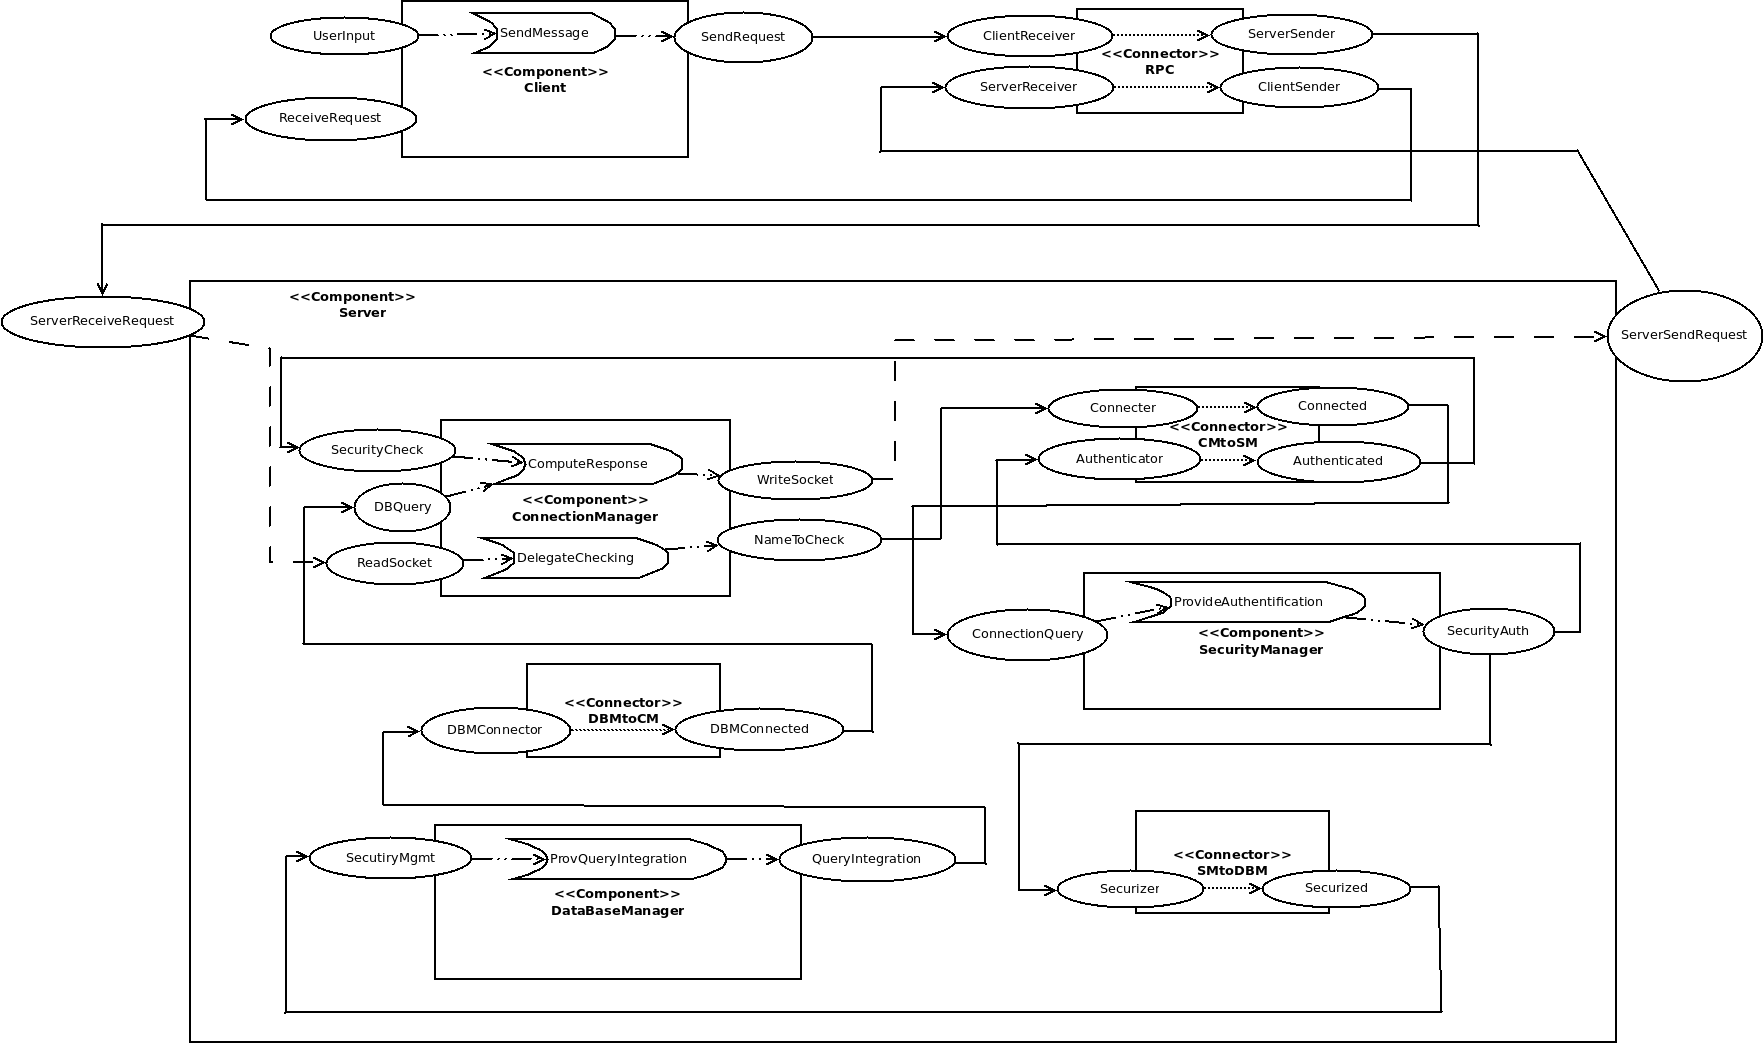
\includegraphics[angle=90,scale=0.5, height=25cm]{Flow.png}
          \caption{Schema de transit des messages}
        \end{figure}
        \FloatBarrier
        
        On peut noter que la propagation s'arrête dans le sous-composant \emph{connectionManager} du server. En effet, il n'y a aucun moyen automatique de passer l'information d'un port requis à un port fourni (pour cela il est nécessaire d'appeler un service).
        
        Afin de continuer l'exécution, et traiter la requête utilisateur, il est nécessaire d'appeler le service \lstinline{delegateCheckingService} du composant \emph{connectionManager}.
        
	\section{Propriétés}
    	L'archive fournie avec ce rapport montre comment utiliser les propriétés dans notre application. Nous avons choisi d'imposer une propriété au niveau de la configuration globale de notre modèle (soit l'application elle-même) : le serveur ne peut pas être attaché à plus d'un client.
        
        Cette propriété n'a évidemment aucun intérêt dans un contexte réel, mais est relativement simple à développer et permet de montrer un exemple concret d'application.
        \newline
        
        La classe \emph{OneServerAttachment} représente cette propriété. La méthode de vérification a été surchargée afin de définir le comportement souhaité. Cette propriété est ensuite ajoutée à la configuration globale via la méthode \lstinline{addProperty(p)}, et sera vérifiée à chaque pas de la propagation.

\addcontentsline{toc}{chapter}{Conclusion}
\chapter*{Conclusion}
	Cette série de travaux pratiques nous a confronté avec les difficultés et ambiguïtés liées à la définition d'un métamodèle d'architecture à base de composants ainsi qu'à son implémentation sous la forme d'un outil.
    \newline
    
    Nous avons fait le choix de développer un outil sous forme de framework, contenant la logique "de base" dans le métamodèle. Cette approche nous semblait la plus adaptée au travail demandée, et permet de créer rapidement et simplement un exemple d'architecture.
    \newline
    
    Cependant, le manque de temps et le grand nombre de projets en parallèle ne nous ont pas permis de mener notre projet jusqu'où nous l'avions initiallement pensé : certaines fonctionnalités sont encore à développer, comprenant entre autres :
    \begin{itemize}
    	\item une fabrique de composants basiques (sans ajout de méthodes au niveau \emph{M1}
        \item des vérification statiques poussées (vérification de cycles de parenté \ldots)
        \item permettre à la glue d'un connecteur d'effectuer un mapping entre les rôle \emph{from} et \emph{to} (dans cette version il n'est possible d'effectuer qu'une fonction d'un rôle vers un autre)
        \item générer une grammaire avec \emph{XText} permettant de définir une architecture par le biais d'un langage déclaratif
        \item etc
    \end{itemize}
    ~\\
    
    Nous restons néanmoins satisfait du travail fourni, et en tirons deux principaux avantages :
    \begin{itemize}
    	\item une meilleure compréhension des architectures à base de composants
        \item un apport non négligeable pour le projet de fin d'études d'extraction d'architecture
    \end{itemize}
	